\chapter{CNIs comparison and assessment}\label{chpt:osu}

This chapter will be entirely dedicated to explaining in detail the criteria and
methodologies adopted to compare the different CNIs analyzed in section
\ref{sec:node2node} to assess their performance and pick the most promising one.

One initial remark that should be remembered throughout the chapter is that all
the tests were performed on a freshly installed Kubernetes cluster with the CNI
plugin under test being initialized with the default configuration.
This means that the results obtained are not necessarily correct in absolute
terms. All the considered options are widely configurable and tunable to fit
specific situations better.

The main idea behind this choice is to pick the option that provides the best
performance out of the box, and then tune it to improve it further.
It could be the case that a discarded CNI could overtake the chosen one with the
proper tuning, but this is out of the scope of this work. This first section
aims to provide a reproducible and reliable comparison method that can be
applied to any Kubernetes cluster to assess the performance of the CNIs under
test. The same methodology could be used again to compare how different
configurations of the same CNI plugin increase or decrease the overall
performance.

\section{Methodology}\label{sec:methodology}

The entire benchmark is based on executing a ping-pong fashion MPI code.
The Message Passing Interface (MPI) \cite{mpi41} is the de-facto standard for
modern parallel programming. It is a specification for a standard library for
message-passing defined by the MPI Forum, a broadly based group of parallel
computer vendors, library writers, and applications specialists. Then, those
standards are applied to many implementations; some are open-source, like
OpenMPI and MPICH, while others are proprietary, such as Intel MPI and IBM
Spectrum MPI.
For this work, the choice of relying on a free and open-source implementation
was made; hence, the final decision fell on OpenMPI, which is widely used and
known in the scientific community.

Although writing an ad-hoc MPI code to perform this ping-pong test should be
relatively easy, opting for a widely used and known benchmark undoubtedly leads
to more comparable results. A well-known benchmark to test the network is the
suite of tests provided by Ohio State University: the OSU Micro-Benchmarks
\cite{osu}.
This suite is a collection of MPI-based benchmarks written in C, Java, or Python
(for this work, only the C version was used) that can be used to measure the
hardware performance of a good variety of network interfaces and network stacks:
InfiniBand, Omni-Path, Ethernet RoCE, and Slingshot.
Although the OSU benchmarks were created to compare the performance of different
hardware, they can also be used in different scenarios, like this case study.
The main idea is to repeat the same test on the same hardware with different CNI
plugins; in this way, it will be possible to provide a quantitative comparison
of the overhead introduced by the different CNIs and the impact on the overall
performance of the cluster.

The process to perform the tests is quite simple: a couple of pods will be
spawned; each pod will contain a container with a copy of the compiled binaries
of the OSU benchmark and a process to run those binaries.
Those two pods will be scheduled both on the same node and then on different
nodes; this can be achieved in Kubernetes with the
\texttt{spec.topologySpreadConstraints} field in the pod definition
\cite{kdoc-topologyconstraints}.

During the initialization of any MPI program, with the function
\texttt{MPI\_Init()}, every process is informed about the existence of the
others, their rank, and most importantly, how to reach them for the needed
communication. In particular, the MPI library achieves the latter by knowing the
other nodes' IP address or a resolvable hostname.
This may be commonplaces in a traditional HPC cluster, where the nodes are all
connected to the same network and the hostname of the nodes is resolvable to the
corresponding IP address. However, in the case of the setting described for
assessing the Kubernetes connectivity plugins, this last part is more complex
than in the traditional HPC scenario.
Containers are isolated from the host and each other, and the hostname of a
container is usually a random string, different at each restart.
Moreover, by definition, each pod has its own Network Namespace. Hence, the IP
address of a container is not reachable from another container unless some
specific configuration is made (like the configuration of a \texttt{service}).

A straightforward solution to this problem is relying on the Kubernetes
\texttt{mpi-operator} developed by the KubeFlow community
\cite{kubeflow-mpioperator}.
This operator acts like a controller which allows to spawn a CRD (Custom
Resource Definition) called \texttt{MPIJob} \cite{redhat-mpioperator} that
creates the pods and sets up the communication between them.
In this way, it should only specify how many replicas of a ``worker'' pod must
be created. The operator will take care of the rest, spawning all of them plus
one (or more) ``launcher'' pod that will submit the job and redirect the
program's output executed by the workers in its logs.
In this way, the programmer can write its MPI code as usual, without worrying
about all the behind-the-scene stuff (SaaS approach), and have the containerized
version of the code running on a Kubernetes cluster.

It was said that two pods would be spawned, each containing a running container
with the OSU benchmark binaries. What remains to be clarified is how such a
container is built.
The entire process, which leads to the final image usable by the MPI operator,
is quite simple and made by some modular steps that can be easily modified to
replace the MPI distribution adopted or the code.
The various steps (schematized in figure \ref{fig:mpi-container-creation}) are:
\begin{itemize}
  \itemsep0em
  \item \textit{Builder container creation}: This container is meant to be used
    only to compile a given MPI-based code. It is just a minimal image (in this
    work, a \texttt{debian:bookworkm} image was used) with the necessary dev
    tools (like \texttt{gcc} and \texttt{make}) and the MPI library installed.

    The idea behind keeping this step isolated from the rest is that in this way,
    once a building pipeline is created, the transition between different
    implementations of the MPI library is straightforward since this is the only
    image that needs to be changed.

  \item \textit{Code provider container creation}: This container is meant to
    provide the MPI code to be executed. It can be a minimal image (for this
    thesis again, a \texttt{debian:bookworkm} image was used) which
    alternatively downloads the code from the internet (e.g., using
    \texttt{curl}/\texttt{wget} or cloning a git repository) alternatively, copy
    it from a mounted volume. In this work, the first approach was used, taking
    the last version of the code\footnote{At the moment of writing: version 7.4
      uploaded on 2024-04-26.} directly from the official site of the Ohio State
    University.
    The idea behind this step is to keep the code separated from the rest of the
    pipeline so that it can be easily changed, keeping the same building pipeline
    for different code with the same compilation system (e.g., \texttt{make \&\&
      make install}).

  \item \textit{code compilation}: intermediate step, in which the builder
    container compiles the code provided by the code provider container. In
    order to exploit the underlying hardware fully, the code was compiled in the
    same node where it would be executed. In this way, the
    compiler can optimize the code for the specific architecture of the node's
    CPU.

  \item \textit{creation of the final image}: In this phase, the binaries
    obtained with the compilation are stored in the final image. This image was
    created as a Debian image with the chosen (OpenMPI) MPI library installed
    and \texttt{openssh} installed and properly configured to allow the
    communication between the different pods for the \texttt{mpiuser} user, as
    the operator would expect.

  \item \textit{execution on the Kubernetes cluster}: using a \texttt{MPIJob}
    CRD, the operator will spawn the pods and execute the code. The code output
    will be redirected to the launcher pod logs so the user can easily check the
    results.
\end{itemize}


\begin{figure}
  \centering
  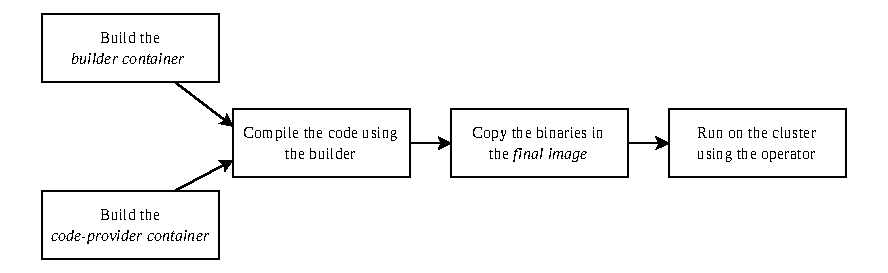
\includegraphics[width=\textwidth]{img/chpt3/mpi-container-building}
  \caption{Synthesis of the process to build a container compliant with the MPI
    operator.}
  \label{fig:mpi-container-creation}
\end{figure}


\subsection{About the OSU Micro Benchmarks}

It was previously said that the OSU Micro Benchmarks are a suite of MPI-based
benchmarks. The suite comprises a good variety of tests, each focusing on a
specific aspect of the network performance.
For this work, all the chosen tests were taken from the \texttt{pt2pt}
(Point-to-Point) category, which contains tests that measure the latency or the
bandwidth between exactly two processes performing a ping-pong test.
In particular, three tests were chosen for assessing the latency and equally for
what concerns the bandwidth. The tests are \cite{osu}:

\begin{itemize}
\itemsep0em
\item \textit{Latency}:
  \begin{enumerate}
    \itemsep0em
    \item \texttt{osu\_latency}: classical ping-pong test measuring the time to
      send and receive back a message of an always increasing size. The blocking
      version of MPI communication functions (\texttt{MPI\_Send} and
      \texttt{MPI\_Recv}) is used.
    \item \texttt{osu\_latency\_mp}: Multi-process Latency test. Similar to the
      previous case, but in this case, both the sender and the receiver
      processes have ore child spawned with a \texttt{fork()} system call. The
      sending process(parent) sends a message of a given data size to the
      receiver(parent) process and waits for a reply from the receiver process
      while the children process sleeps for 2 seconds after the fork call and
      then exits.
    \item \texttt{osu\_multi\_lat}: Multi-pair Latency test. In this case,
      processes simultaneously perform a sending operation on each other.
      Instead of being a classical ping-pong test, this is a ping-ping test.
  \end{enumerate}
\item \textit{Bandwidth}:
  \begin{enumerate}
    \itemsep0em
    \item \texttt{osu\_bw}: The test has a sender process that sends a message of
      a given size to the receiver process and waits for the receiver to answer
      (it will do it after all the data has been received).
      This process is repeated several times, and the time elapsed is recorded.
      The bandwidth is calculated as the maximum amount of data that can be
      exchanged in a given block size for a given time.
      For this test, the non-blocking version of the MPI communication functions
      (\texttt{MPI\_Isend} and \texttt{MPI\_Irecv}) is used.
    \item \texttt{osu\_bibw}: Bidirectional Bandwidth test. It is analogous to the
      previous test, except that, in this case, both processes send and receive
      data simultaneously.
    \item \texttt{osu\_mbw\_mr}: Multiple Bandwidth test. Similar to the simple
      uni-directional bandwidth test, but in this case multiple pairs of
      % new line because the long tt-string was going out of the page
      processes are created, like in the \\ \texttt{osu\_latency\_mp} case.
  \end{enumerate}
\end{itemize}


The execution of each of these benchmark will be repeated 30 times, in order to
guarantee a statistical significance of the results.

\section{How measurements were conducted}\label{sec:measurements}

First of all, a premise to keep in mind during the continuation of this entire
thesis. The expression \textit{``bare metal''} will be adopted to refer to the
case of operation executed out of the scope of the Kubernetes container
orchestrator. More precisely, the expression will refer to the case when the
code is executed directly on the node, allocating resources in a traditional HPC
approach, asking them to the resource manager (in this case, SLURM), and
avoiding using containers.

\subsection{Used hardware}\label{subsec:hardware}

To perform (almost\footnote{See Appendix \ref{appendix:kprod} for more detail}),
all the tests described in this chapter and in the chapter \ref{chpt:dask} were
performed on the same hardware.
The available resources assigned to the investigation project of this thesis
consist of a cluster of 3 nodes from the THIN partition of the ORFEO cluster.
Each of these nodes (they are all identical in any aspect) is equipped with two
\texttt{Intel Xeon Gold 6126} processors; each of those CPUs is composed of 12
cores with a base frequency of 2.6 GHz and a maximum turbo frequency of 3.7 GHz.
The total amount of RAM available per node is 768 GB (12x64 GB 2666 MT/s), which
composes two NUMA regions, one for each socket. The available hyper-threading
was disabled, hence every time in this work the concept of core will be
mentioned, it will be refers to physical core.

The nodes dispose of a 25 Gbps Ethernet network card, which serves two ethernet
ports connected to the same switch. InfiniBand was also available on those nodes
but was not used for the tests.
The reason behind this choice is that the examined CNI, unlike the Mellanox
CNis, does not support, at least out of the box, the InfiniBand network. To
guarantee a fair comparison, the tests were performed enforcing the usage of the
ethernet connection, even in the bare metal scenario where InfiniBand was
available.


\subsection{Used software}

All the nodes were uniformly configured with the same software stack to avoid
possible data distortion. The operating system was freshly installed using
Cobbler (a Linux installation automation tool for servers) to avoid any possible
interference with previous installations.
The software stack was composed by the components listed in table
\ref{tab:softwarestack}.

\begin{table}[H]
  \centering
  \begin{tabularx}{\linewidth}{p{0.225\textwidth}p{0.225\textwidth}X}  % Correct environment and column specification
    \toprule
    \textbf{Component} & \textbf{Name \& Version} & \textbf{Notes} \\
    \midrule
    O.S.              & \texttt{Fedora 40}           & Linux kernel: \texttt{9.12-200.fc40.x86\_64} \\
    Compiler          & \texttt{gcc 14.2.1 20240801} & \texttt{(Red Hat 14.2.1-1)}   \\
    MPI library       & \texttt{OpenMPI 4.1.6rc4}    &  \\
    Python            & \texttt{Python 3.11.9}       & Directly compiled on the nodes using the \newline \texttt{-}\texttt{-enable-optimizations} flag. \\
    Resource manager  & \texttt{SLURM 24.05.2}       & Used for the ``bare metal'' measurements \\
    Container runtime & \texttt{cri-o 1.28.2}        &  \\
    Kubernetes        & \texttt{k8s 1.30.4}          &  1 control plane node, 2 worker nodes\\
    CNI-plugins       & \texttt{Calico 3.28.0}       & Installed with the \texttt{tigera-operator 1.34} \\
    \                 & \texttt{Cilium 0.16.15}      & Installed with the \texttt{cilium install} command \\
                      & \texttt{Flannel 0.25.4}      & Installed through a manifest which pulls the \texttt{docker.io/flannel/Flannel:v0.25.4} image. \\
    MPI Operator      & \texttt{0.5.0}               &  \\
    Dask Operator     & \texttt{2024.7.1}            & Needed for Dask tests presented in chapter \ref{chpt:dask} \\
   \bottomrule
  \end{tabularx}
  \caption{Summary of the software stack used for the tests. All the components
    were installed on the nodes uniformly using the latest stable version
    available at the time of writing. The CNIs were installed one at a time,
    rebooting the node between the installation of the different plugins to
    avoid any possible interference.}
  \label{tab:softwarestack}
\end{table}

\section{Results}\label{sec:cniresuls}

Since the results of the tests are pretty extensive, in order to avoid the
cluttering the text, only a brief summary of the results will be provided,
taking one example for each category of tests (latency and bandwidth) to give an
idea of the results obtained, which will be reported in this section.

For the sake of completeness, the results of all the tests are available in a
dedicated report that was not attached to this thesis for its size.
The report is available in the public repository of the thesis at the following link:

\begin{center}
  \small
  \url{
    https://github.com/IsacPasianotto/master-thesis/blob/main/appendixB-osu_results/report.pdf
  }.
\end{center}

Moreover, to help the reader to follow the results, all the numerical results
presented graphically in this section are available in the appendix \ref{appendix:osu}.

\subsection{Latency}\label{subsec:results-latency}

In figures \ref{fig:latency-mp-1-node} and \ref{fig:latency-mp-2-nodes} are reported
the results of the \texttt{osu\_latency\_mp} test performed on a single node
(\ref{fig:latency-mp-1-node}) and on two nodes (\ref{fig:latency-mp-2-nodes}).
Both the configurations allows to draw interesting conclusions.

Let's start the analysis from the single node case
\ref{fig:latency-mp-1-node}\footnote{Data are available in tables
  \ref{tab:latency-mp-baremetal-1nodes}, \ref{tab:latency-mp-calico-1nodes},
  \ref{tab:latency-mp-cilium-1nodes}, and \ref{tab:latency-mp-flannel-1nodes} at
  appendix \ref{appendix:osu}.}.
A marked difference between the bare metal case and all the CNI cases is
immediately noted. This might lead to premature conclusions that communication
within the same node is immeasurably slower than in the bare metal case.
However, some considerations must be made to avoid any hasty misinterpretation.
This notable difference (about two orders of magnitude) is due to the fact that
under the hood, two very different scenarios are being compared.
In the case of bare metal, the communication between two processes, which are
aware that they are running on the same node, has a very low latency. In fact,
the communication is done through shared memory, with no interaction with all
the system parts involved in inter-node communication.
On the other side, when two MPI processes are spawned in two different
containers in two different pods, from the processes' point of view, they will
act as if they are on two different nodes since they are not aware of the actual
underlying infrastructure.
This phenomenon is well appreciable if we compare the results of the latency in
Kubernetes of the communication between two pods on the same node and the one on
two different nodes. In figure \ref{fig:cilium-latency} is reported as an
example of the case with the Cilium CNI.
The plot highlights how the two latency measurements are, at least for a small
number of bytes sent and received, on the same order of magnitude, while in the
bare metal case, the difference is hugely more expansive. This difference in the
behavior is the consequence of what was previously explained: while in the bare
metal case, the communication is done through shared memory, hence the
transition from the single node to the multi-node involves a change in the
communication protocol, in the Kubernetes case the communication is done through
the same mechanisms, so the difference between the single and multi-node case is
entirely due to the slow down introduced by the physical network the message has
to travel through.

However, this does not mean that these results are pointless; on the contrary,
they are very convenient in understanding the overhead the CNI plugin
introduces, with no other external factors that could interfere with the
results, like the actual usage of the network.
We can see that thanks to its kernel-level approach, the Cilium CNI plugin
introduces the lowest overhead. At the same time, flannel, probably due to the
encapsulation/decapsulation process that the packets have to undergo, is the one
that performs the worst.
This means that Cilium should provide the lowest latency in communication
between two pods scheduled on the same node in the Kubernetes cluster among the
considered candidates.

It is not the primary goal of this benchmark to assess the absolute performance
of the containerized implementation of the bare metal scenario. However, since
this entire thesis is dedicated to studying if a cloud-native infrastructure can
be used to perform HPC-like tasks, an important consideration must be made: the
presented setting does not guarantee, but also does not claim to do so, the best
performance that can be achieved with the bare metal scenario.
To do so, using only one bigger container and spawning all the MPI processes
inside is more convenient. This way, the communication between the processes
will be done through shared memory, and the latency will be very low, at the
point that the results are not distinguishable for the bare metal
case\footnote{See table
  \ref{tab:latency-mp-one-pod} in appendix \ref{appendix:osu} for
  quantitative results.}.
The communication between pods in the same node is meant for applications whose
workflows are not highly coupled and for which the tolerance threshold for the
latency is higher. If this is not the case and performance is the priority,
hence putting the various components of an application in different pods is
logically wrong, and the best choice is to use a single pod with all the needed
containers inside. In this way, all the processes will be able to communicate
through a shared memory without the need to consult Kubernetes to know how to
reach each other (recall that all the resources in the same pod share the
network namespace).


\begin{figure}
  \centering
  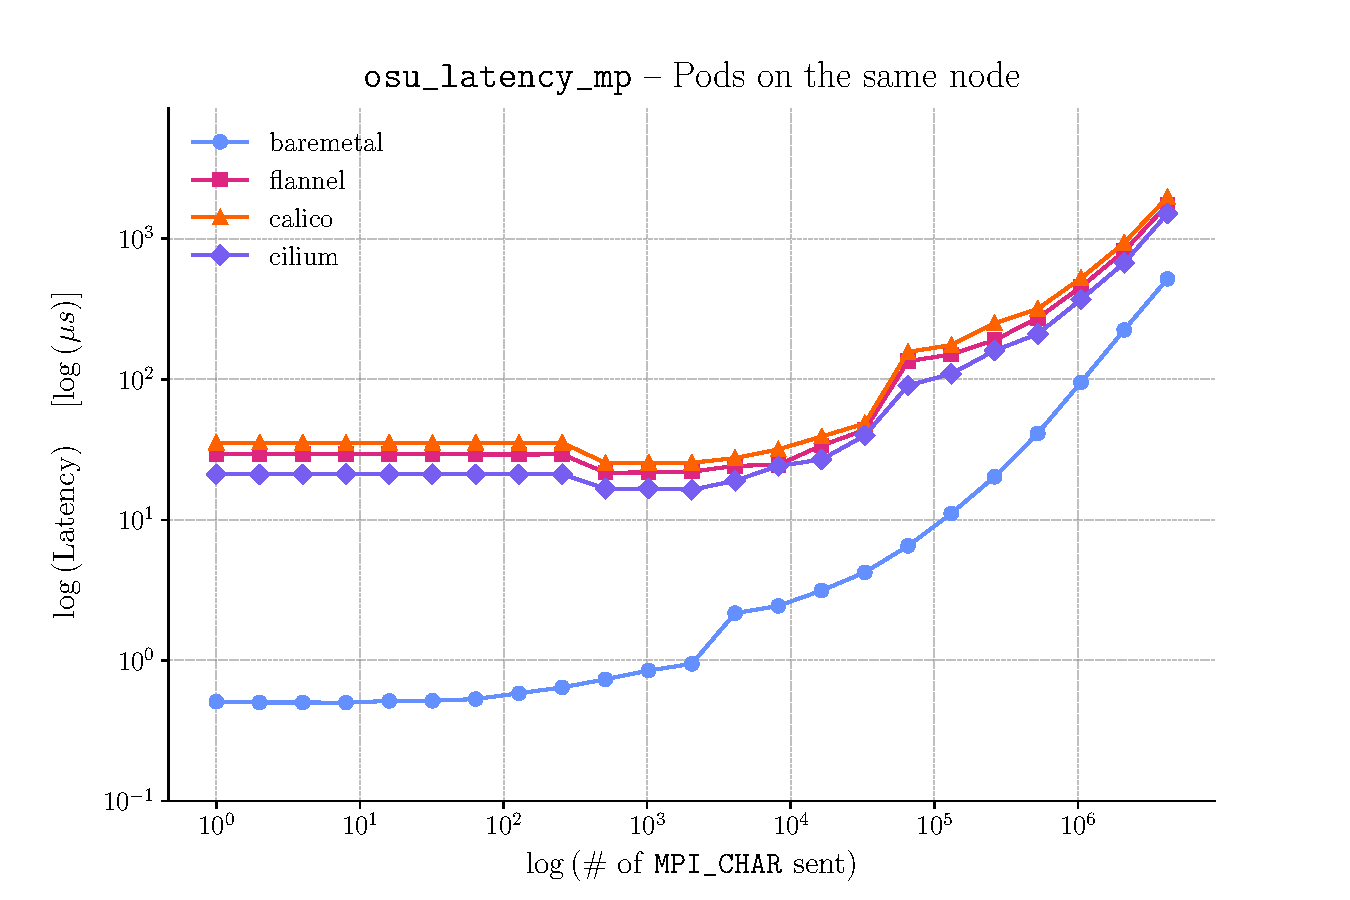
\includegraphics[width=0.94\textwidth]{img/chpt3/latency_mp-1-node}
  \caption{Result of the \texttt{osu\_latency\_mp} benchmark performed on a single
    node; the lower the better.}
  \label{fig:latency-mp-1-node}
\end{figure}


\begin{figure}
  \centering
  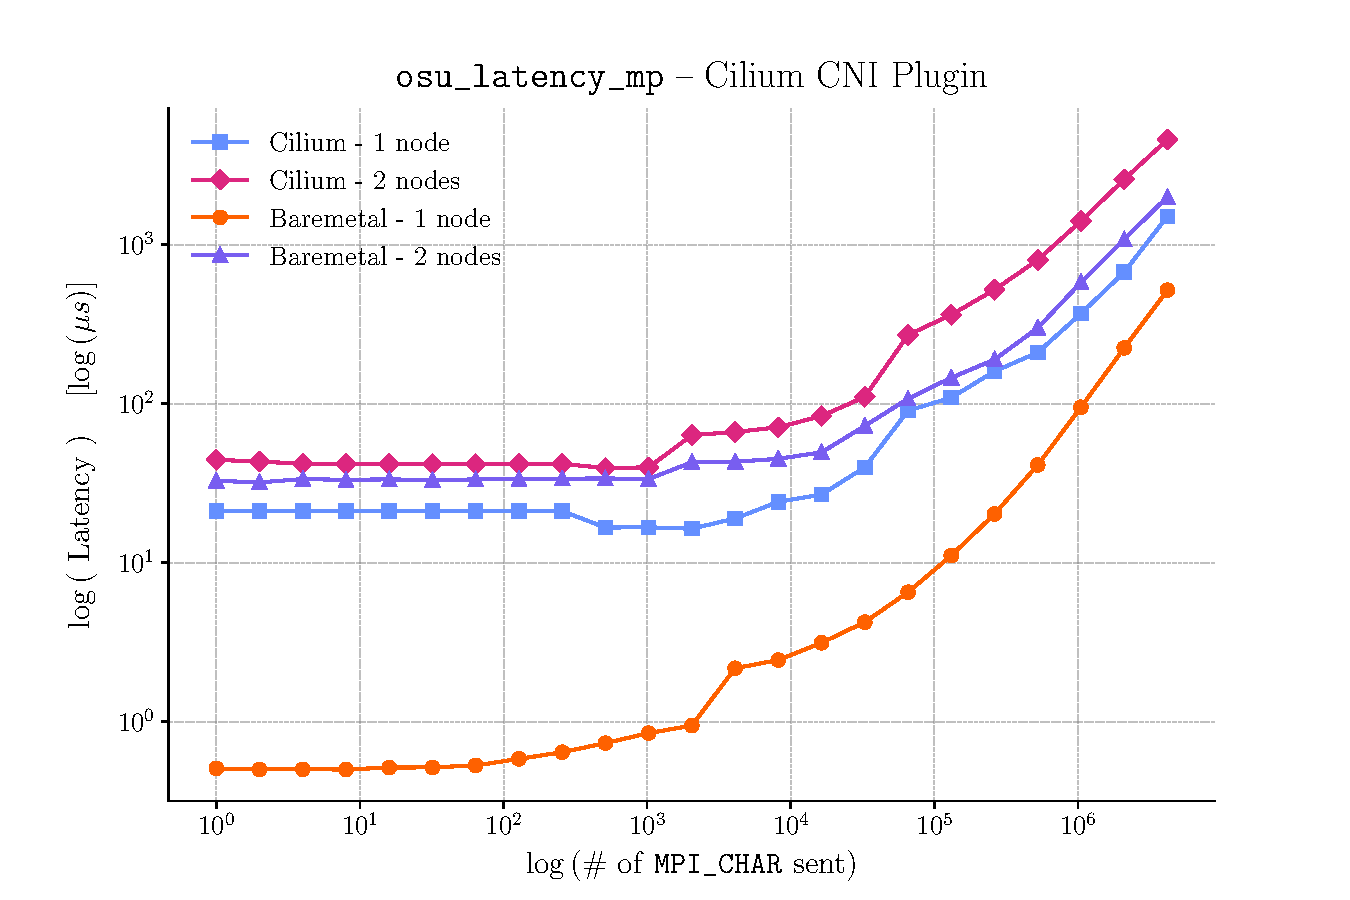
\includegraphics[width=0.94\textwidth]{img/chpt3/cilium-latency_mp}
  \caption{Comparison of the \texttt{osu\_latency\_mp} results for the Cilium
    CNI plugin.}
  \label{fig:cilium-latency}
\end{figure}

The situation is quite different when communication is performed among different nodes.
In this case, see figure \ref{fig:latency-mp-2-nodes}\footnote{Data are available in tables
  \ref{tab:latency-mp-baremetal-2nodes}, \ref{tab:latency-mp-calico-2nodes},
  \ref{tab:latency-mp-cilium-2nodes}, and \ref{tab:latency-mp-flannel-2nodes} at
  appendix \ref{appendix:osu}.},
All the measurements are closer to each other and have the same magnitude.
In this situation, the comparison is more ``fair'' since all the communication
takes place through the network, letting the data show the price paid in terms
of latency for the overhead introduced by each CNI plugin.
Flannel confirms his tendency to be the slowest CNI plugin, while the duel
between Calico and Cilium is not a clear winner. The eBPF based is clearly
faster for small messages, while the BGP-routing strategy seems to reward more
at the increase of the message size and, starting from the \texttt{262144
  MPI\_CHAR} message size beats Cilium with a lower latency.
However, it must be said that the gap between Calico and Cilium for bigger
message sizes is much less broad than the same distance in small messages.
This should be taken into account when reasoning in terms of a general-purpose
infrastructure with no particular hints about the kind of workload that will be
commonly executed on it.

In general, the results of the latency tests are pretty interesting and
allows to be optimistic about the possibility of using a Kubernetes cluster to
perform HPC-like tasks.

\begin{figure}
  \centering
  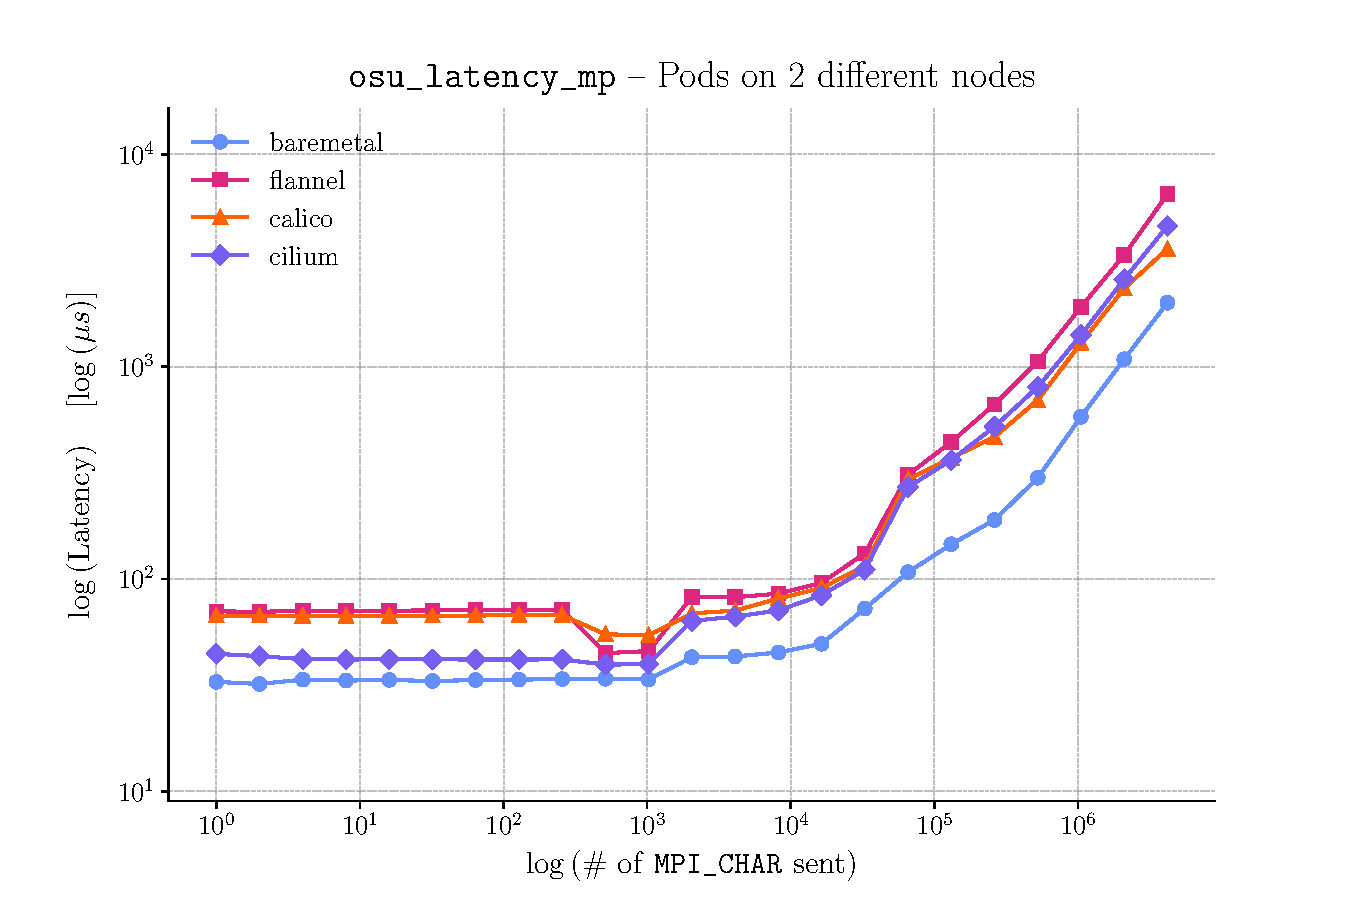
\includegraphics[width=0.94\textwidth]{img/chpt3/latency_mp-2-nodes}
  \caption{Result of the \texttt{osu\_latency\_mp} benchmark performed on two
    nodes; the lower the better.}
  \label{fig:latency-mp-2-nodes}
\end{figure}

% Accordingly how LaTeX render this part comment or not that:
\clearpage

\subsection{Bandwidth}\label{subsec:results-bandwidth}

Alongside latency, another vital aspect to consider when assessing the
performance of a network is bandwidth.
Like in the previous section, in figure \ref{fig:bibw-1-node} and
\ref{fig:bibw-2-nodes} are reported the results of the \texttt{osu\_bibw}
benchmark performed on a single node (\ref{fig:bibw-1-node}) and on two nodes
(\ref{fig:bibw-2-nodes})\footnote{
  Data for the one node case can be consulted in
  tables \ref{tab:bibw-baremetal-1nodes}, \ref{tab:bibw-calico-1nodes},
  \ref{tab:bibw-flannel-1nodes}, and \ref{tab:bibw-cilium-1nodes}, while data
  for the two nodes case are available in tables
  \ref{tab:bibw-baremetal-2nodes}, \ref{tab:bibw-calico-2nodes},
  \ref{tab:bibw-flannel-2nodes}, and \ref{tab:bibw-cilium-2nodes} at appendix
  \ref{appendix:osu}.
}.

Regarding the single node case, considerations similar to the one made for the
latency case can be made about the gap between the bare metal case and all the
Kubernetes cases.
In this case, the difference between the different solutions still not be vast
enough to discard a priori a certain CNI plugin; however, what is interesting to
note is that also, in this case, there is always a best performer (Cilium), and
a worst one (Calico) independently from the message size.

\begin{figure}
  \centering
  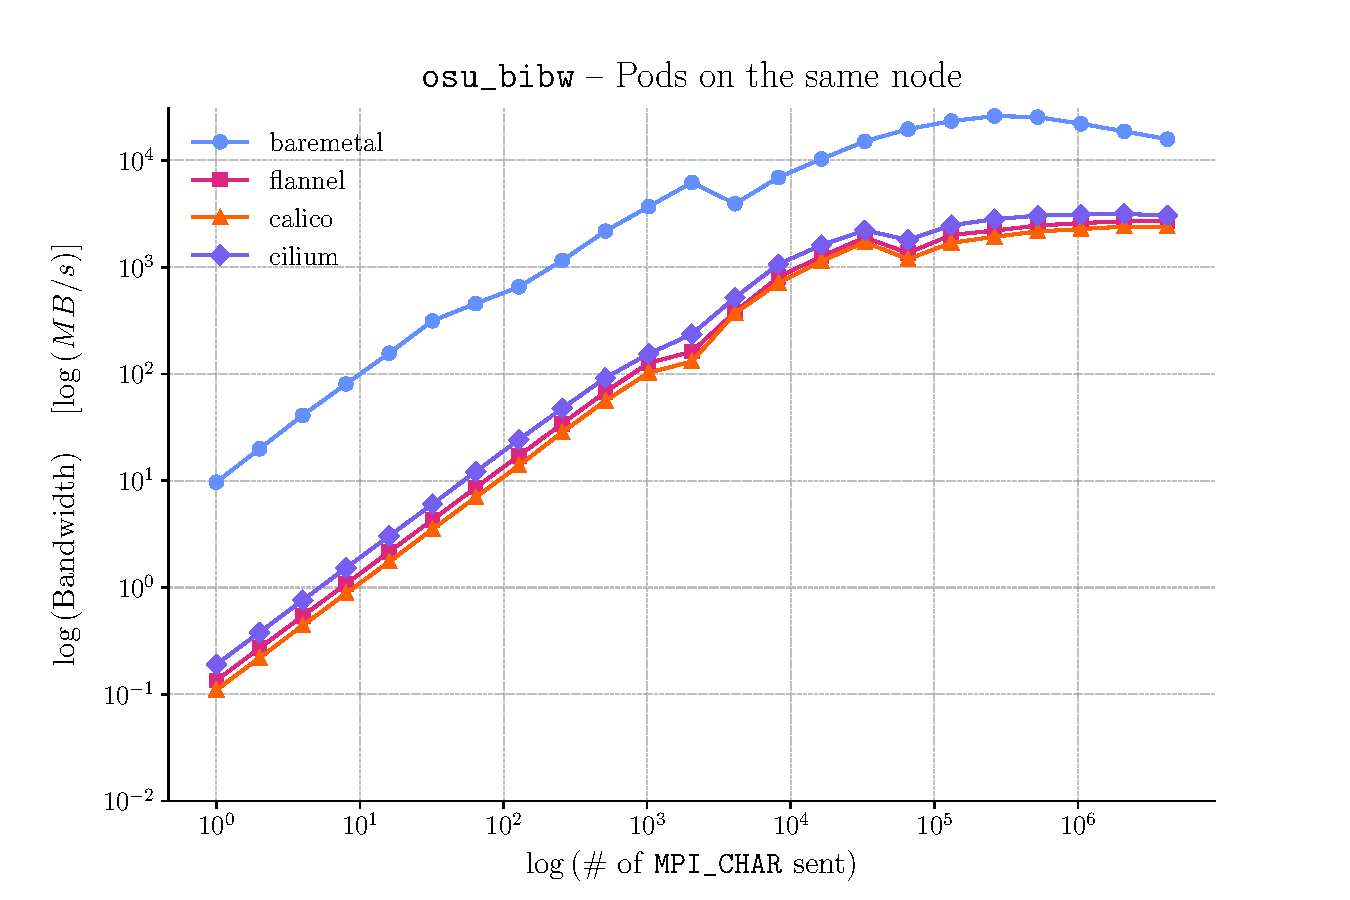
\includegraphics[width=0.94\textwidth]{img/chpt3/bibw-1-node}
  \caption{Result of the \texttt{osu\_bibw} benchmark performed on a single
    node; the higher the better.}
  \label{fig:bibw-1-node}
\end{figure}

The analysis of the other case (inter-node communication) is also fascinating.
Once again, the Cilium CNI outperforms the other candidate for small-size
messages, reaching a bandwidth extremely close to the bare metal case.
Similar to the previous case, the BGP routing strategy of the Calico CNI plugin
appears to be the least convenient way to saturate the network, resulting in the
slowest independent form of the message size.
Flannel starts performing poorly for small messages. However, as the message
size increases, the overhead introduced by the encapsulation/decapsulation
process remains constant, making it more negligible and letting the plugin
overtake Cilium for more prominent messages.

% \begin{figure}
\begin{figure}[H]
  \centering
  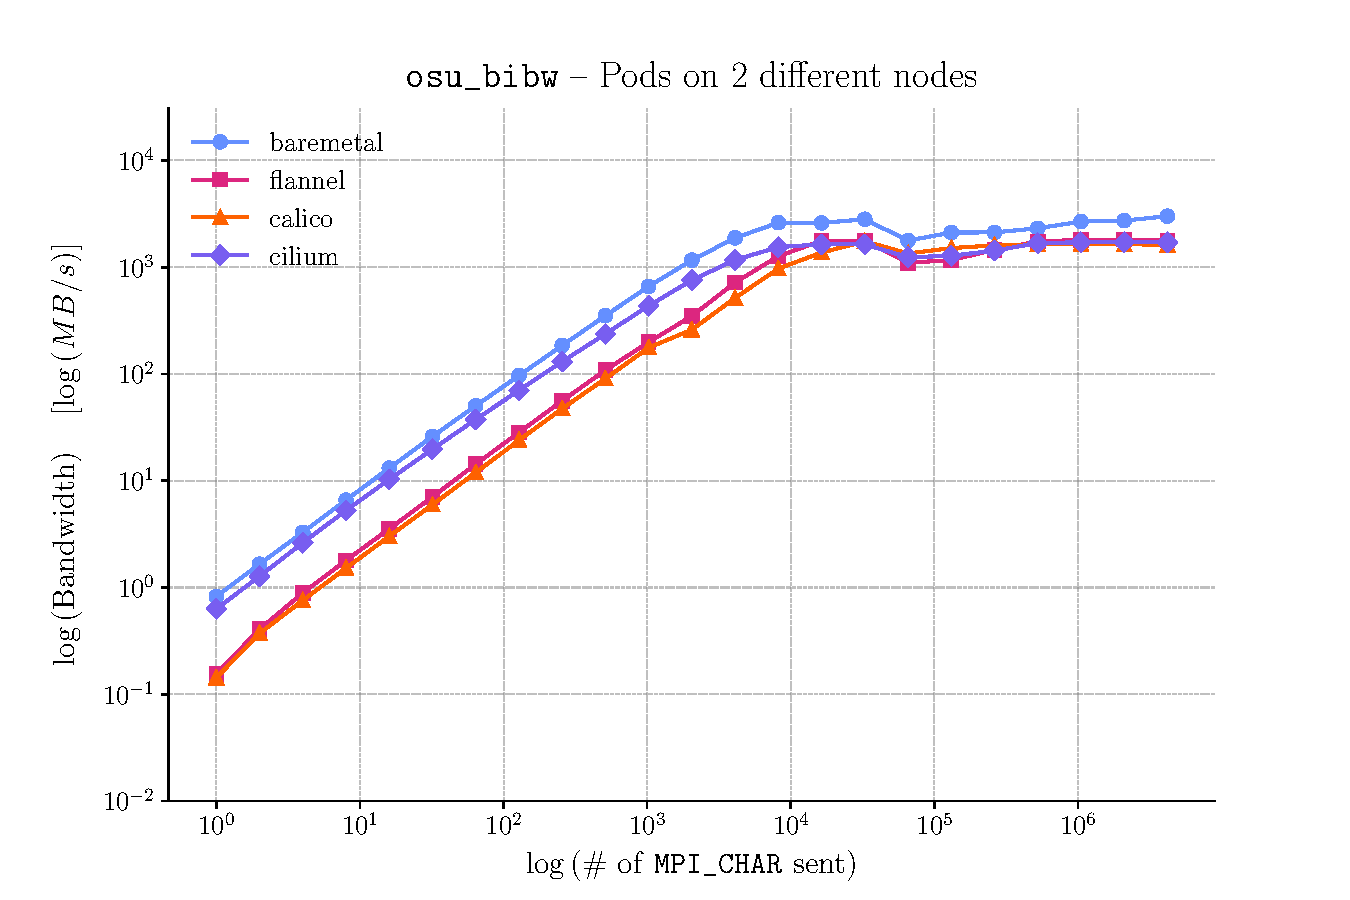
\includegraphics[width=0.94\textwidth]{img/chpt3/bibw-2-nodes}
  \caption{Result of the \texttt{osu\_bibw} benchmark performed on two nodes; the
    higher the better.}
  \label{fig:bibw-2-nodes}
\end{figure}

\section{Final considerations}\label{sec:final-considerations}

The results of the measurements conducted in this chapter led to the final
decision to adopt the Cilium CNI plugin as the most promising candidate for the
infrastructure this thesis claims to deploy for the execution of HPC-like tasks.
The choice was made primarily considering the fact that this plugin was never
the more mediocre one in any of the tests performed.

Flannel was the CNI plugin that delivered the highest bandwidth in multi-node
communication (the most critical and common scenario in any HPC-like
application). However, his latency performance was less satisfying independently
from the message size, up to the point that it doubled/triplicated the time to
perform the same ping pong test compared to the bare-metal case.
In addition, the lack of official, well-structured documentation and the
necessity of relying only on community support made the choice of Flannel the
less appetitive one and the first to be discarded.

Calico, on the other side, was the solution that won the competition for the
multi-node test latency at the end of the message size spectrum, but it was
arguably the worst performer for the bandwidth test.
However, this superior performance in latency is significant only for huge
message size (greater than 1 MB), which may not be enough to justify all the
costs in terms of bandwidth that the plugin introduces, and the more significant
latency in smaller messages.

Since no detailed assumption was made about the kind of HPC workloads that will
be executed on the infrastructure (like distribution of message sizes
frequency), it can be considered wise to adopt the more balanced solution, which
is the Cilium CNI plugin.
Despite not being the best performer for a more significant number of exchanged
bytes, it was always the second best with a minimal gap from the winner.
Moreover, in the situations in which it was the best performer, which are the
small messages and all the cases of intra-node communication, the difference
concerning the bare metal case was far less than the other CNIs, which means
that the overhead introduced by the plugin is minimal.

In addition to that, the Cilium project has a well-structured and complete
documentation, which can be very useful in solving any possible issue and tuning
the configuration to perform even better than the out-of-the-box configuration.
Even if it alone is not a sufficient reason to choose a solution, it is worth
mentioning that together with his eBPF-based CNI plugin, the Cilium project
deliver also a handy command line tool, invokable via the \texttt{cilium}
command, which can be used to monitor, configure, and troubleshoot the network
effortlessly and intuitively making the management less painful and more
efficient.

For all these reasons, the Cilium CNI plugin was chosen as the most promising
candidate to be used in the infrastructure object of this thesis, and it will be
the CNI plugin used in the next chapter to show a case of study of a complete
parallel code execution on the Kubernetes cluster.

It must said that the results obtained, despite being quite encouraging,
highlights that an approach like the one proposed in this thesis to use a
container orchestrator to perform HPC-like tasks from a strictly
performance-focused point of view can be considered a step back from the
traditional systems labeled bare metal in this discussion.
Considering the chosen CNI plugin, Cilium, the pick of the bandwidth reached
1711.73 MB/s, which is just over half of the 3006.66 MB/s obtainable by
scheduling the same code on the same hardware with SLURM.
The case of the latency is analog, where the 44.37 $\mu$s are a third more than
the 32.75 $\mu$s obtainable with the traditional approach, and the gap gets
wider as the number of exchanged bytes increases: 4588.27 $\mu$s against the
1998.00 $\mu$s of the baseline for 4194304 \texttt{MPI\_CHAR}.

However, as seen in sections \ref{sec:chpt1-orchestrator} and
\ref{sec:chpt1-kubernetes}, the Kubernetes orchestrator brings many benefits
that can be worth the slight loss in performance.
In particular, the autoscaling feature can be handy in a scenario where the
workload is not constant and can vary a lot in time, overcoming the rigidity of
the traditional resource allocation in which the resources are asked at the
beginning of the job and are kept until the end, even if they are not needed
anymore.

While in the case of an HTC (High Throughput Computing) workload, this slight
loss in network performance is absolutely acceptable, since the parallelization
is done performing multiple independent tasks, and the communication between the
independent worker is minimal, a more careful evaluation is needed in the cases
in which the communication between the workers is more frequent, and the
tolerance threshold for the latency is lower.

The next chapter, chapter \ref{chpt:dask}, will show an example of a complete
simulation of workloads typical in modern distributed computation frameworks,
with the intent of investigating if the tradeoff between all the benefits the
Kubernetes orchestrator brings as a scheduler and the slight loss in performance
is worth or not.

